\section{Results}
\label{sec:results}

\subsection{Power Comparisons}
\label{sub:power_comparisons}

Figure~\ref{fig:simulatedGeneRealData} displays the mean empirical power for each test under various scenarios for the 50 randomly selected genes.
In each scenario I considered a single causal region of size $\gamma$.
The size of the causal region was defined relative to the total gene size (given in percentage).
For example, given a gene with 10 rare variants and $\gamma=0.2$ then the first $2$ mutations defined as causal mutations.
Empirical power was compared between Skat, SkatO, KS, CMC, Burden and KS-Burden under different assumed effect sizes ($r^2=(0.002, 0.006, 0.009)$).
The selected $50$ genes had at least $6$ genetic variants and maximal $60$ with a median of $8.5$ variants.

All tests were affected by the size of the causal cluster.
As expected, KS and Skat greatly lose statistical power when $\gamma$ increases.
The KS test showed greater statistical power between $\gamma=0.2$ and $\gamma=0.6$ than Skat, but lost significant power when $\gamma$ increases.
Further, KS performed only slightly better than Skat at $\gamma=0.2$.
Interestingly the simple KS test also outperformed SkatO at $\gamma=0.4$, but to a lesser extend.
Both burden tests, that is CMC and Burden, demonstrated an monotonic increase in statistical power over $\gamma$.
Thus suffering from a reduction in power at $\gamma=0.2$ but outperformed all other tests when all variants were disease causing.

Omnibus tests, that is SkatO and KS-Burden, are relatively unaffected by the change in $\gamma$ and KS-Burden is able to outperform SkatO across scenarios.
However, while the mean power of SkatO remains rather stable across all scenarios, KS-Burden has a slight reduction in power at $\gamma=0.2$.

Assessment of the correlation between test statistics of KS and Burden test across assessed genes under the null was with $r=0.03$ small.
Thus providing some evidence for the indecency of both tests. %TODO need to check this correlation again 

\begin{figure}[ht!]
  \centering
  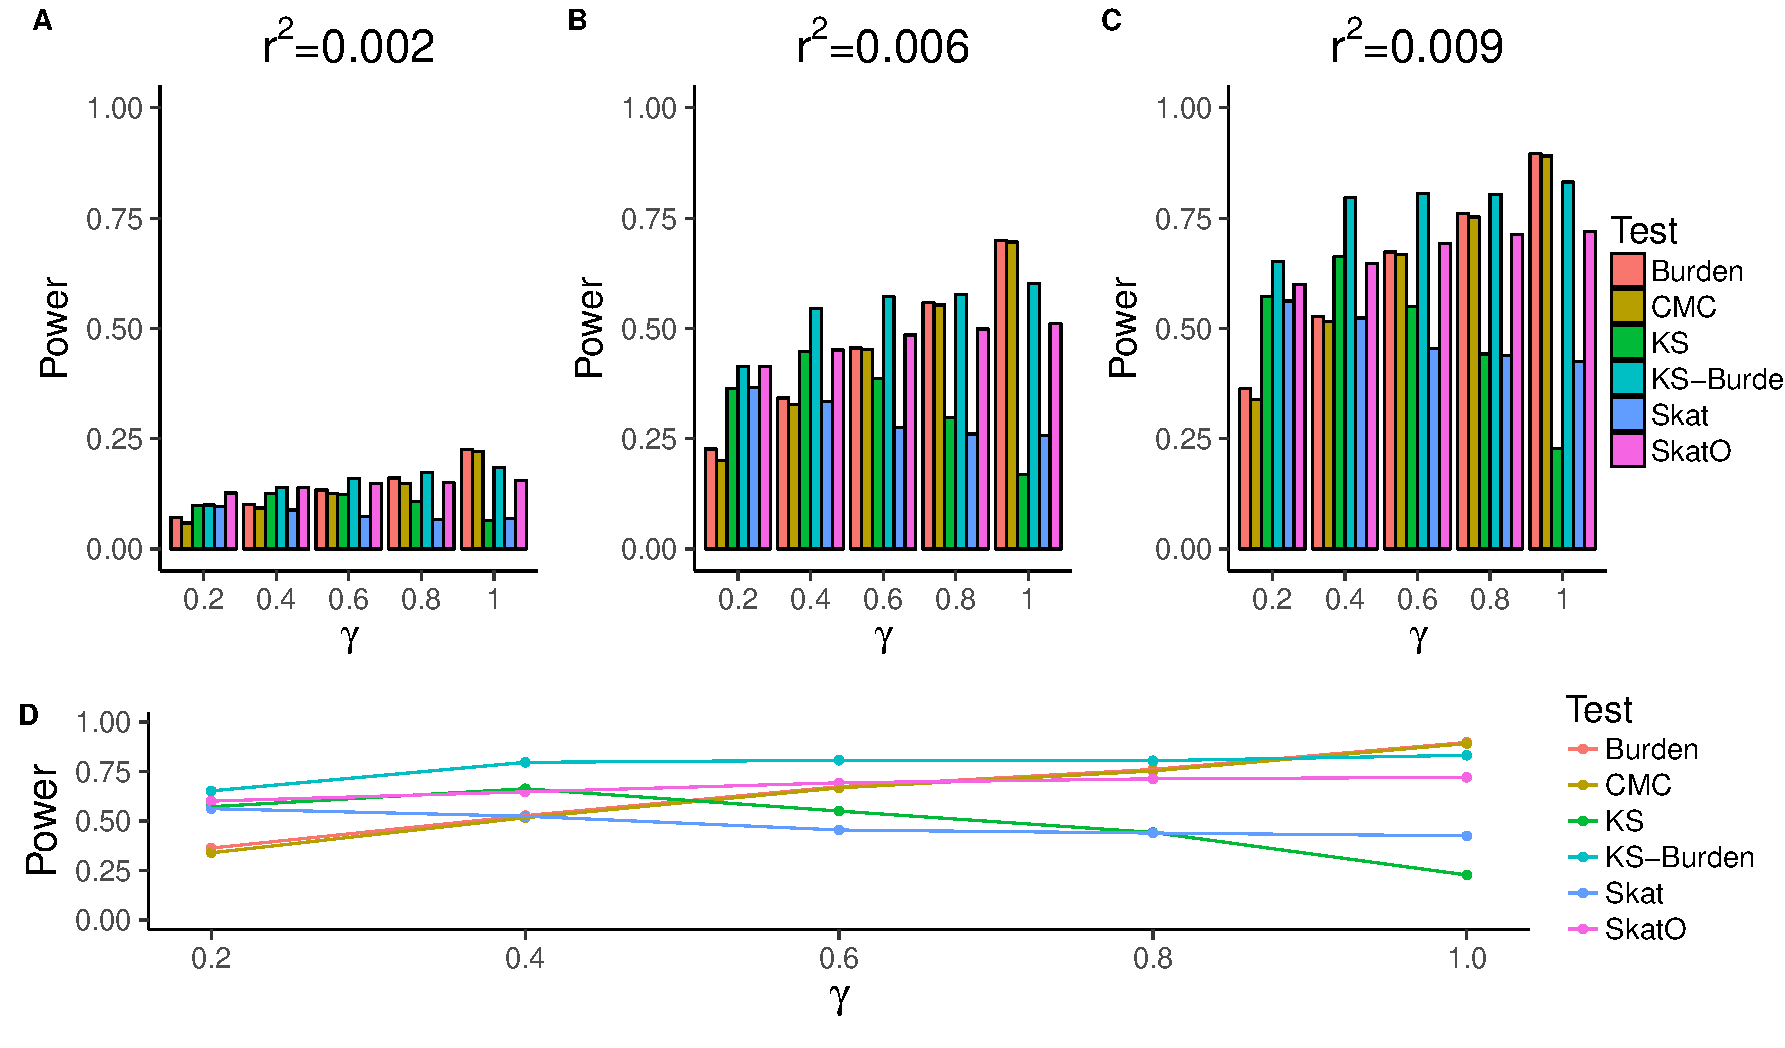
\includegraphics[width=1.0\linewidth]{ksburden/figures/combined_power_analysis.pdf}
  \caption[Estimated mean statistical power]{Estimated mean statistical power for five different causal cluster size $\gamma$ over selected 50 genes.
    (A--C) Different power estiamtions for each rare variant association test for $r^2=0.002, 0.006, 0.009$.
    The percentage of causal mutations $\gamma$ are on the corresponding x-axis, while empirical power is on the y-axis.
    (D) Relative change in empirical power over changes in $\gamma$ for each assessed test.\label{fig:simulatedGeneRealData}}
\end{figure}


\subsection{UK BioBank -- Aggression}
\label{sub:ukbiobank_aggression}

Following I applied the KS-Burden test on the UK BioBank in order to identify genes enriched for, as well as distributrional differences of rare mutations. 
The KS-Burden test was unable to identify any genes significant assocaited with impulsive aggression (see Table~\ref{tab:top_ksburden}).
Inspection of the QQ-plot (see Figure~\ref{fig:qqplot_ksburden}) further suggests the absence of any signal within the tested phenotype.

\begin{figure}
  \begin{floatrow}
    \ffigbox[7cm]{%
      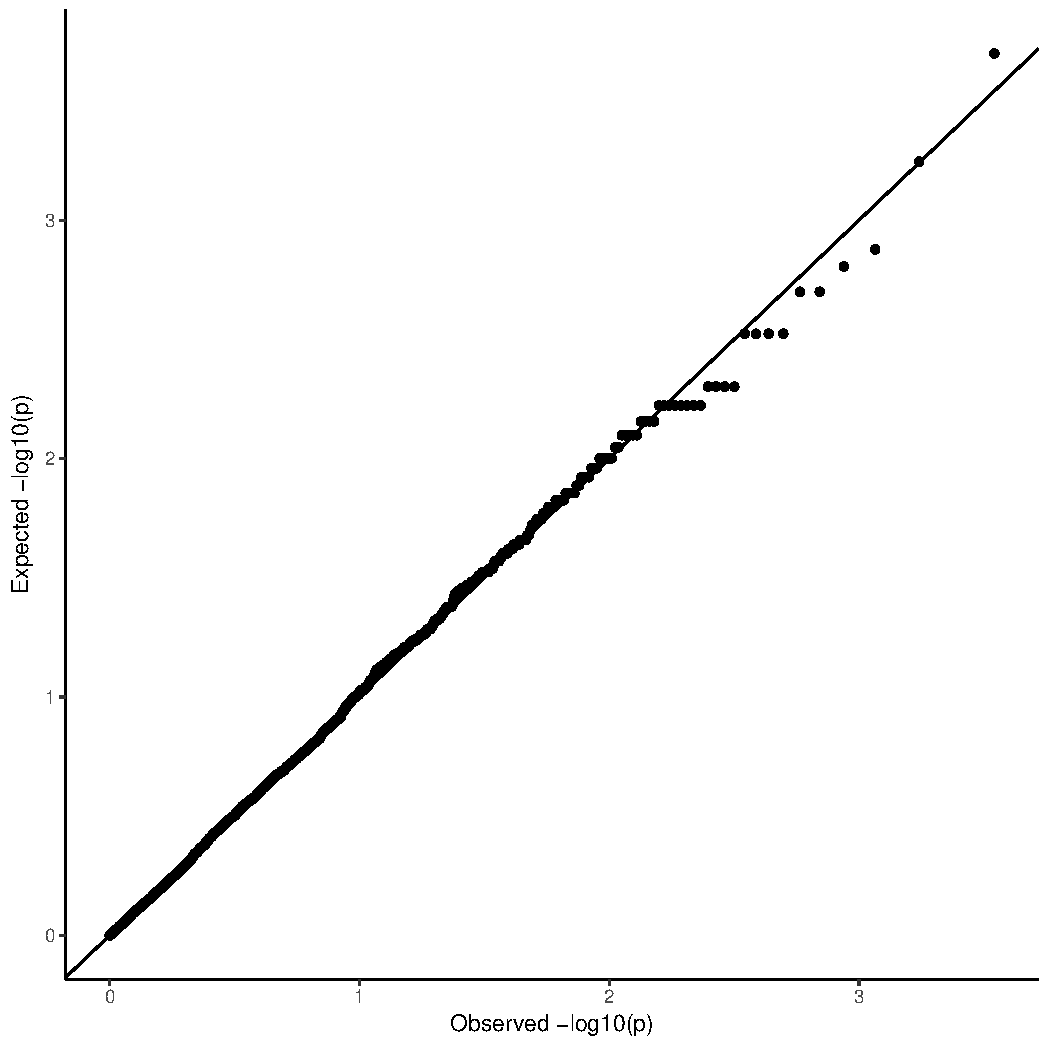
\includegraphics[width=0.5\linewidth]{ksburden/figures/qqplot_aggression.pdf}
      }{%
      \caption[QQ-plot of KS-Burden Test]{QQ-plot of KS-Burden Test.}\label{fig:qqplot_ksburden}
    }
    \capbtabbox[7cm]{%
      \resizebox{7cm}{!}{%latex.default(tab, title = "", file = "UKB_aggression_results.tex",     rowname = NULL, digits = 3)%
\begin{tabular}{lrrr}
\hline\hline
\multicolumn{1}{c}{Gene}&\multicolumn{1}{c}{KS-Burden}&\multicolumn{1}{c}{KS-Burden(FDR)}&\multicolumn{1}{c}{No.Var}\tabularnewline
\hline
PJA2&$0.000170$&$0.419$&$3$\tabularnewline
ANKRD12&$0.000341$&$0.419$&$4$\tabularnewline
TANC2&$0.000361$&$0.419$&$5$\tabularnewline
ADGRA3&$0.000615$&$0.506$&$5$\tabularnewline
NCF2&$0.000906$&$0.506$&$3$\tabularnewline
AHSG&$0.001043$&$0.506$&$3$\tabularnewline
APOBEC3F&$0.001187$&$0.506$&$5$\tabularnewline
LRRC71&$0.001266$&$0.506$&$5$\tabularnewline
SLC7A4&$0.001309$&$0.506$&$3$\tabularnewline
LEMD1&$0.001615$&$0.562$&$3$\tabularnewline
\hline
\end{tabular}
}
      }{%
      \caption[KS-Burden Results]{
        Top 10 Genes based on the KS-Burden Test.
      Number of variants present in each given gene are indicated in the last column (No.Var)}\label{tab:top_ksburden}
    }
  \end{floatrow}
\end{figure}
